% !TeX root = ../Thesis.tex
\chapter{Fundamentals}

\section{HippoCampus $\mu$AUV Platform}

\subsection{Hardware}
\begin{figure}[h!]
    \centering
    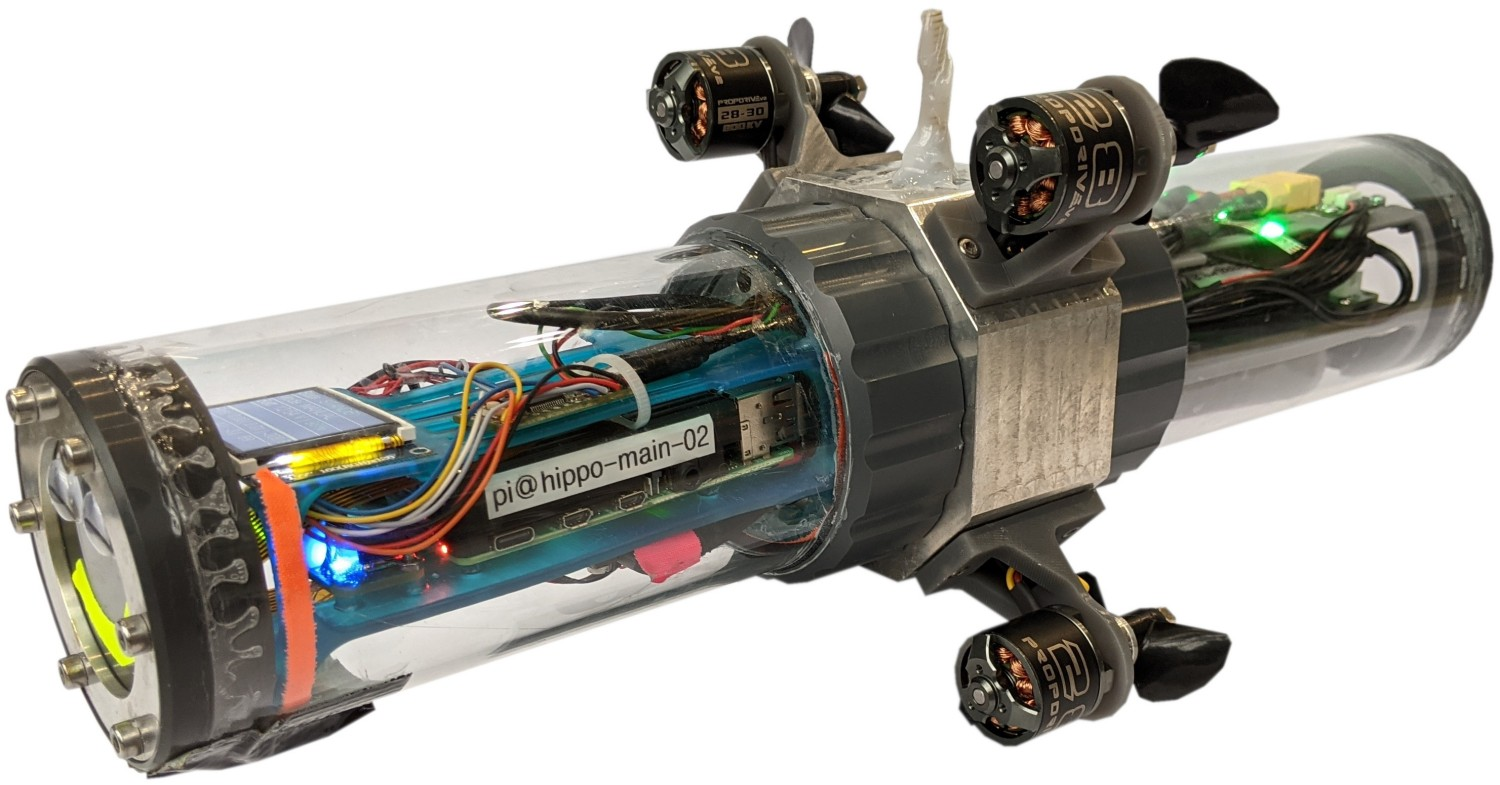
\includegraphics[width=0.4\textwidth]{hippo_picture}
    \quad\quad
    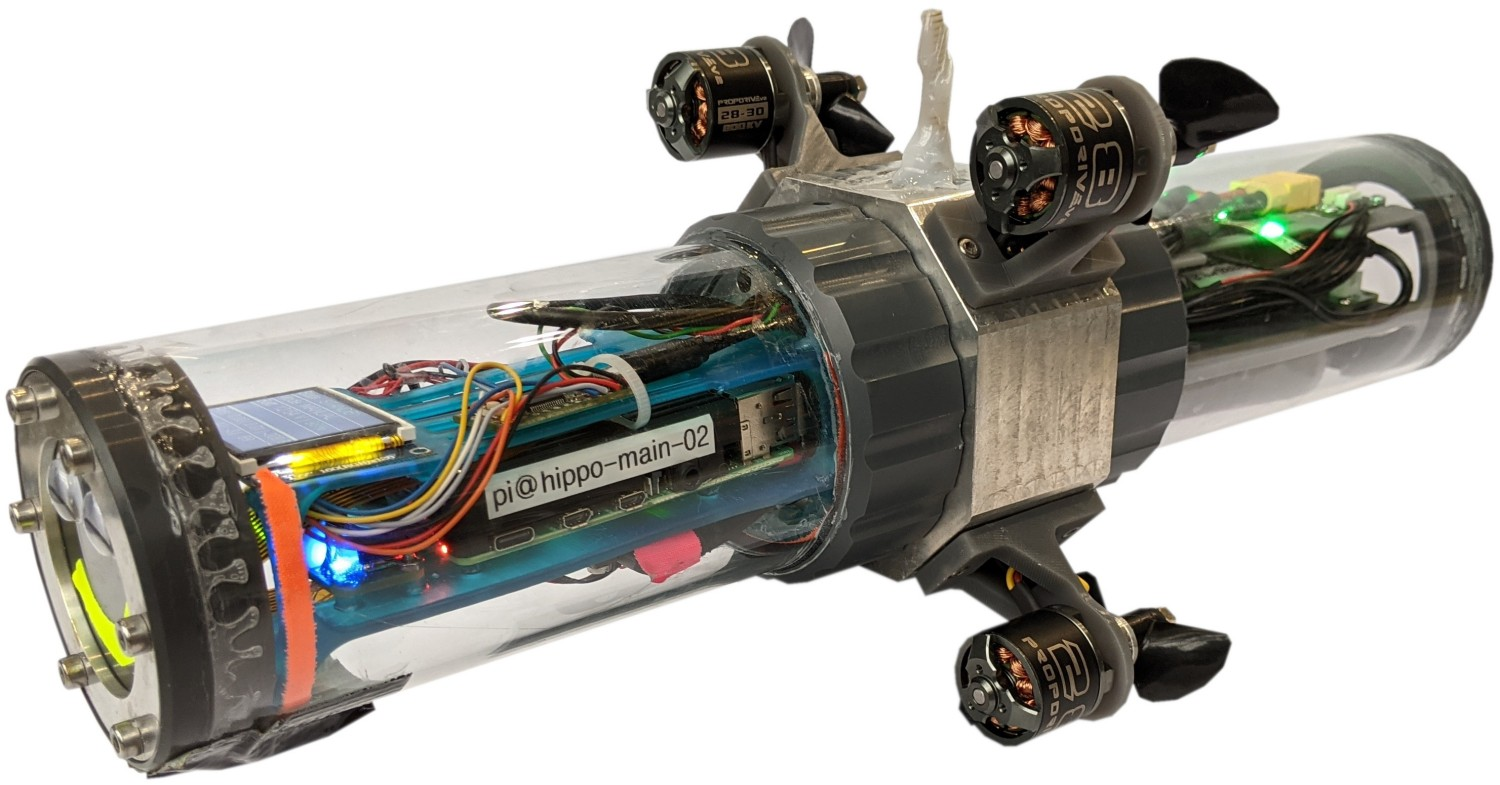
\includegraphics[width=0.4\textwidth]{hippo_picture}
    \caption{\textcolor{blue}{HippoCampus $\mu$AUV in its heavy configuration (\textit{left}) and redesigned version based on BlueRobotics off-the-shelf components (\textit{right}).} \textcolor{red}{reference in text}}
    \label{}
\end{figure}
\subsection{Software-Architecture}
\begin{figure}[h!]
	\centering
     \def\svgwidth{12cm}  
	\input{images/02/03_hippo_system_architecture_draft.pdf_tex}
	\caption{System architecture of the HippoCampus $\mu$AUV.}
\end{figure}

\begin{figure}[h!]
	\centering
    \def\svgwidth{12cm}  
	\input{images/02/03_sw_layer.pdf_tex}
	\caption{Software-Architecture with multiple layers of abstraction facilitating vertical
and horizontal extensions. \textcolor{red}{adapt and say something about MAVROS / uORB etc pp}}
\end{figure}

\section{Review on Motion Planning}
\label{sec:review-motion-planning}
\subsection{Underwater Motion Planning}
\begin{itemize}
    \color{red}
    \item \cite{Panda20} for review on auv path planning
\end{itemize}
\label{sec:underwater-motion-planning}
We refer to motion planning as either path planning or trajectory planning. Path planning only considers the spatial aspect of motion, while for trajectories there is a relation between the geometric path and time. Often, it is convenient to decouple the path planning aspect from the temporal planning. By assigning a velocity profile to the planned path, a trajectory can be obtained after the path planning problem is solved. Hence, no rigorous distinction between trajectory and path planning is made in the course of this section.

In the following, a selection of widely used algorithms for solving underwater path planning problems is introduced, their concept briefly summarized and example applications in the domain of \acp{auv} presented. This should provide a sufficient overview of the state of the art, to discuss strengths and limitations of existing underwater path planning methods.

\cite{Panda20} presents a comprehensive overview of various path planning approaches for single- or multi-\acsp{auv} scenarios. Since multiagent systems are not the focus of this thesis, the interested reader may refer to \cite{Panda20} for more information on this topic.

%  \cite{Gomez15} classifies different path planning methods: geometric methods, graph- and tree-based methods and artificial potential fields methods. For this thesis, the categorization by the used techniques seems less useful than grouping the methods by their field of application.

\subsubsection{Graph- and tree-based Methods}
According to \cite{Gomez15}, methods falling in this category are subject to the highest research effort during recent years. Well known and often used algorithms belong to this group of path planning methods, such as A*, \ac{rrt} or \ac{fmm}.


\paragraph{Grid-based Search}
For grid-based approaches like A*, the vehicle states or the environment are discretized and encoded as nodes in a graph, building the search space. Costs are assigned to the edges connecting the nodes. Depending on the used algorithm, a path is searched, that connects the initial state with a desired goal state.
To obtain, for example, the shortest path, the costs can be defined as the euclidean distance between discrete positions in the environmet. The  nodes of the graph encode the discretized environment.
Subsequently, a search algorithm guaranteeing optimality can be deployed to find the path with the lowest costs, if one exists. Due to dicretization, accuracy is decreased. A smaller grid size counteracts this problem, but increases the search space and therefore the computational costs for finding a solution.

The authors in \cite{Fernandes2015TowardsAO} declare A* in its generic form as general not suitable for mobile robots with time constraints, due to the performance costs associated with traversing the state space if replanning is required. Still, there exist various publications applying variants of A* in the context of path planning for mobile robots and \acp{auv} in particular.

Applications of A* in the domain of \acp{auv} go back to the 90s \cite{Carroll92}, while still being extended in recent works \cite{zhang20}. Common to these approaches is the application for oceanic environments, where obstacles are assumed to be static, traveled distances to be large, and vehicle dynamics not to be relevant.

\paragraph{Sampling-based Search}

A typical representative of sampling-based methods is \ac{rrt}. Even though, the original version of \ac{rrt} does not provide optimality, it compensates for that by being able to efficiently solve complex planning problems, that are possibly high-dimensional \cite{Devaurs16}. Randomly sampled points are connected to generate a tree to find a path between initial and goal state.

In \cite{Young13} the authors present a path planning approach based on \ac{rrt} for \acp{auv} in the presence of obstacles. Kinematic constraints, such that the vehicle can only move with certain velocity limits are respected. A model for the hydrodynamic properties of the vehicle is not considered, though.

The problem of non-optimality is addressed in \cite{Karaman11} with a modification of \ac{rrt}, called anytime \ac{rrt}, though not applied in the underwater domain. The idea is, to find a solution as fast as possible and improve the solution if given further computation time. This renders the approach especially useful for dynamic environments.

An informed variant of \ac{rrt}, called RRT*, is used in \cite{Ma18} for terrain-aided navigation for long range navigation of \acp{auv}.



\subsubsection{A*}
\subsubsection{FM*}
\cite{Petres09}
\begin{itemize}
    \color{red}
    \item Combination of Fast Marching and A*
    \item can constrain curvature (useful for traditional/torpedo shaped uuvs.)
\end{itemize}
\subsubsection{Potential Fields}
\subsubsection{Model Predictive Control}
\subsubsection{Discussion}
\begin{itemize}
    \color{red}
    \item Vehicles are large/slow
    \item Have more computational power or algorithm in general not real timecapable.
\end{itemize}

\subsection{Review on Agile Path Planning Methods}
\begin{itemize}
    \color{red}
    \item Natural to look at quadrocopters to transfer solutions to the underwater domain because of the similarity of the design.
\end{itemize}
\subsection{Discussion}


\begin{landscape}
\begin{table}[]
%\renewcommand{\arraystretch}{1.0}
    \caption{Overview on ....}
		%\hspace*{-1.5cm}  % move table down (left in landscape) - tabular width: 
		\centering
		% change column width: >{\hsize=1.5\hsize\linewidth=\hsize}
		% >{\hsize=0.5\hsize\linewidth=\hsize}
		\begin{NiceTabular}
            {
            %%%%% Leider scheint die beste Methode wirklich hardgecodete Spaltenbreiten zu sein - hier am Ende rumspielen
            >{\scriptsize\centering\arraybackslash}m{1.7cm} % Method
            >{\scriptsize\centering\arraybackslash}m{1.2cm} % 
            >{\centering\scriptsize\arraybackslash}m{3cm}   %
            >{\centering\scriptsize\arraybackslash}m{3cm}   % 
            >{\centering\scriptsize\arraybackslash}m{3.2cm} % 
            }
            \toprule
            %%%%%%%%%%% Top row - names of each columns
            Method
            &  Spalte 2
            &  Spalte 3
            & Spalte 4
            & Spalte 5 \\  
            \midrule 
            
            %%%%%%%% Beispiel
            Bla bla \cite{MuellerHehn15}
            & test
            & bla 
            & bla 
            & test
            \\ 
            \bottomrule
		\end{NiceTabular}
		\label{tab:state_of_the_art}
\end{table}
\end{landscape}

